\chapter{Satellite Constellation Management Tools} \label{chapter_tools}
This chapter presents all the tools developed along this work to achieve the purposes of the thesis.

\section{Orbit Propagators}
Applications and topics covered by this thesis clearly require an orbital propagator to be studied.
All the propagators produced along this work exploit the Cowell's model shown in subsection \ref{orbit_prop_paragraph}.
Both undisturbed and perturbed motion have been analysed.

Orbit propagators must take in input the following data:
\begin{itemize}
    \item \textbf{Initial orbit}. The initial state of the staellite orbit must be defined before propagation.
          All the six orbital elements (see subsection \ref{sat_state_rep_paragraph}) and the epoch are required. 
          The scripts can also work defining the six components of position and velocity vectors.
          Even the TLE can be set as input, which will be appropriately converted into the classical elements representation.  
    \item \textbf{Spacecraft specifications}. According to the features of the selected propagator, one or more satellite characteristics shall be provided when considering perturbations.
          For instance, in presence of atmospheric drag, $C_D$ and $BC$ (which means cross-sectional area and mass) are needed. 
          The reflectivity coefficient must be added if the problem takes into account the SRP.
    \item \textbf{Time settings}. These input parameters include \textit{time frame} and \textit{time step}.
          The first one simply consists of the total temporal period of propagation requested by the user.
          On the other hand, the time step is strictly related to the output accuracy.
          Lower values imply more accurate results, as well as longer computation times.
          In a nutshell, the outputs will be discretized in as many points as those deriving from the ratio between time frame and time step.
          The accuracy of the model is actually always the same. 
          The difference lies in the shape of the outputs: small time steps provide narrower plots. 
          Figure \ref{time_step_fig} shows the SMA of a LEO satellite propagated for one orbit that lasts approximately 50 minutes. The assigned time step is of 5 minutes (the curve is therefore discretized into 10 points).
    \item \textbf{Perturbations parameters}. Propagators that involve any perturbing acceleration need the parameters which describe that force. 
          For example, the perturbing specific force of atmospheric drag (equation \ref{eq:drag_acc}) requires the air density, which will be given by a specific atmospheric model.
          Even for the acceleration of an eventual thruster it is necessary to specify the force it generates.
\end{itemize}

\begin{figure}[h]
      \centering
      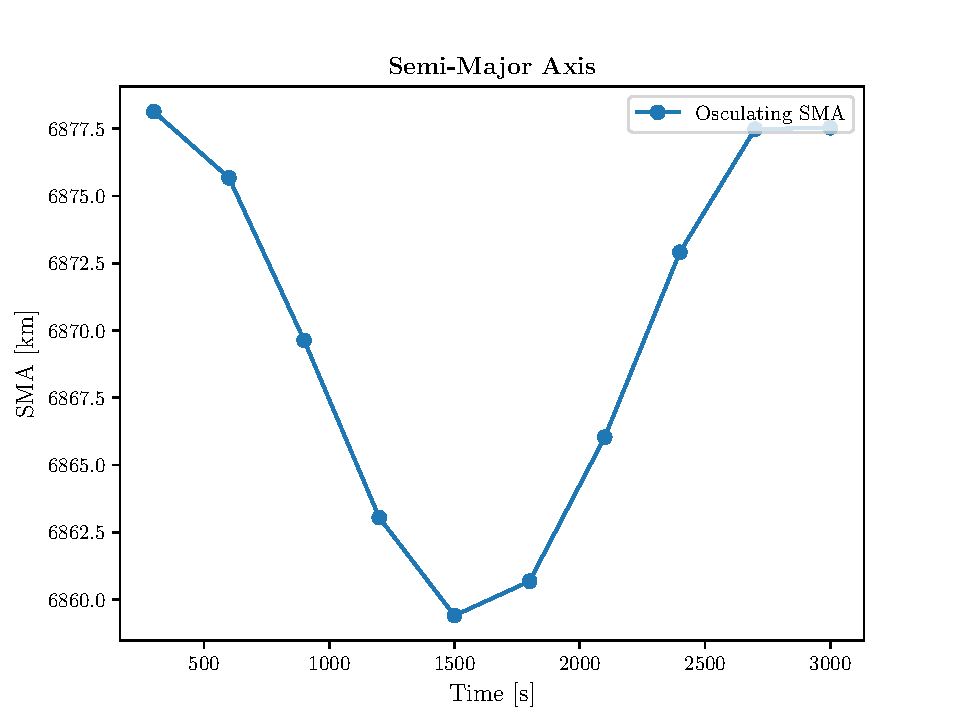
\includegraphics[scale=0.9]{img/time_step.pdf}
      \caption{Osculating SMA output plot of a LEO satellite during one orbit (\textit{time step = 5 minutes, time frame = 50 minutes}).}
      \label{time_step_fig}
  \end{figure}

\subsection{Undisturbed Motion}
The first orbit propagator proposed by this thesis consists of the ideal motion of a spacecraft neglecting all the possible perturbation that might affect it.
Therefore, the only force acting on the body derives from the Earth's gravity (equation \ref{kepler_eq}).
\begin{equation} \label{kepler_eq}
      \ddot{\vec{r}} + \frac{\mu}{r^3}\vec{r} = 0
\end{equation}
This model is mainly useful for two reasons.
First, it requires computation times definitely shorter than a perturbed propagation, allowing quick results when perturbations are not 


\subsection{Perturbations}
\subsection{Atmospheric Models}
\subsection{Mean Orbital Elements Converter}
\subsection{Sun Synchronous Orbits Functions}
\subsection{Satellite Constellation Propagator}

\section{Revisit Time Collector}

\section{Station-Keeping Simulator}

\section{Differential Drag Algorithm}